\chapter{Machine Translation}
This chapter describes the classical or start-of-the-art machine translation models from statistical machine translation model to neural machine model. The relative research works on unsupervised machine translation will also be included.


\section{Statistical Machine Translation}
%%%
%The initial models for machine translation are based on words as units (Word-based machine translation), that can be translated, inserted, dropped and reordered.
%Fertility is the notion that input words produce a specific number of output words in the output language.
%
%Define the phrase-based statistical machine translation model mathematically.  First apply the Bayes rule to invert the translation direction and integrate a language model $p_{LM}$ so the best English translation for the input sentence ${f} $ is defined as 
%
%The advantages of the phrase-based machine translation is :
%\begin{enumerate}
%	\item many-to-many translation can handle non-compositional phrase	
%	\item better utilization of local context in translation
%	\item the more data, the longer phrases can be learned 
%\end{enumerate}
Statistical machine translation has achieved success until the beginning of this century. The initial statistical models for machine translation are based on words as atomic units that may be translated, inserted, dropped and reordered. In statistical machine translation, we use both a translation model and a language model which ensures fluent output. Later the statistical machine translation prefers to use translation of phrases as atomic units. These phrases are any contiguous sequences of words, not necessarily linguistic entities. In this approach, the input sentence is broken up into a sequence of phrases, these phrases are mapped one-to-one to output phrases, which may be reordered.

\subsection{Word-Based Model}
\noindent \textbf{Noisy-channel model:}
Noisy channel model based on the notion of a noisy channel from Shannon's information theory has been applied to many language processing problems. Assume the source sentence is a distorted message omitted from the target sentence, we have a model on  how the message is distorted (translation model $Pr(f_1^J|e_1^I)$) and also a model on which original messages are probable (language model ${Pr(e_1^I)}$), our task is to find the best translation ${e_1^I}$ for an input foreign sentence.
\begin{align*}
\argmax{e_1^I} \{Pr(e_1^I | f_1^J)\} & = \argmax{e_1^I} {\frac{Pr(f_1^J | e_1^I)Pr(e_1^I)}{Pr(f_1^J)}} \\
& = \argmax{e_1^I} { \{ Pr(f_1^J | e_1^I) \cdot  Pr(e_1^I)\} }
\end{align*} 

The basic model for word-based model is noisy-channel model. The task of word alignment is an artifact of word-based machine translation. Alignment models target at the reordering problem for word-based translation.\\
\noindent \textbf{Alignment model}: The position $j$ in the source sentence is aligned with the position $i$ in the target sentence when translating, denoted as  ${i=a_j}$. Alignment model is a global reordering model.For whole sentence, we denote the alignment as 
\[a_1^J:= a_1\cdots a_J\]
\subsubsection{Zero-Order Models: IBM-1 \& IBM-2 Models}

We reformulate the translation model with alignment:
\[ Pr(f_1^J | e_1^I) = \sum_{a_1^J} {Pr(f_1^J, a_1^J | e_1^I)}\]
Further decomposed into a length model, alignment model and a lexicon model. 
\begin{align*}
	Pr(f_1^J, a_1^J |e_1^I) = & Pr(J|e_1^I) \cdot Pr(f_1^J, a_1^J | J, e_1^I) \\
	& = Pr(J|e_1^I) \cdot Pr(a_1^J | J, e_1^J) \cdot Pr(f_1^J | a_1^J, J, e_1^I)
\end{align*}

\noindent Assumptions for IBM1 and IBM2 models:
\begin{itemize}
	\item length model
	dependent only on length of target sentence: \[Pr(J|e_1^I) = P(J|I)\]
	\item alignment model 
	dependent only on absolute position and sentence length:
	\[Pr(a_1^J | J, e_1^J) = \prod_{j=1}^J p(a_j|j, I, J)  \]
	\item lexicon model
	dependent on aligned words only:
	\[Pr(f_1^J | a_1^J, J, e_1^I) = p(f_j | e_{a_j})\] 
\end{itemize}
Difference by alignment model:
\begin{itemize}
	\item IBM-1 model: uniform probabilities: ${p(i|j, I,J) = \frac{1}{I+1}}$
	\item IBM-2 model: ${p(i|j,I,J)}$ is a large table which can be initialized by IBM-1 model
\end{itemize}


 IBM-1 model consider all possible reordering as the same possibility.  More often than not that, the word translation for input source word also follows the translation of the predecessor of that word, or more generally in limited distance.  In IBM-2 model, we add an explicit model for alignment.


\subsubsection{First-Order Model: HMM}
Assume $a_j$ depends on immediate predecessor position ${a_{j-1}}$ as in speech recognition:
\[Pr(a_1^J | J, e_1^J) = \prod_{j}^J p(a_j|a_{j-1}, I, J)  \]
\subsubsection{Weighted Model}
To overcome shortcomings in modeling, introduce scaling exponents ${\lambda_{m}}$ as in speech recognition:
\[ Q(f_1^J, e_1^I; a_1^J) = P(J|I)^{\lambda_1} \cdot \prod_{i} P(e_i|e_h)^{\lambda_2} \cdot \prod_{j} [p(a_j|a_{j-1}, I, J)^{\lambda_{3}} \cdot p(f_j|e_{a_j})^{\lambda_4}]  \]
where $e_h$ denotes the history words in $N$-gram model

\subsubsection{Fertility: IBM-3 Model}
 Mostly, one word in the source language corresponding to just one single word in the target sentence. But fertility models that each source word can be translated to zero or more than one words.\\
\textbf{Fertility}  models $\varphi(e)$ the specific number of target words given an source word $e$. As consequence, length $J$ depends on fertilities:
\[ J = \sum_{i=0}^I \varphi(e_i)\]
Since fertility models the one-to-many translation or dropping input words.  Similarly, we need to model adding words. IBM models these added words are generated by the special NULL token. We could model the fertility of the NULL token in the same way. After fertility step,  we insert one NULL token with a specific probability $p$ after each generated word. \\

IBM-3 model contains four steps: 
\begin{itemize}
	\item fertility step
	\item NULL insertion
	\item lexical translation step
	\item distortion step for reordering
\end{itemize}

\subsection{Phrase-Based Model}
Actually when translating, words may not be the best candidates for the smallest units for translation, sometimes one word in a foreign languages should be translated into two English words, or vice versa. Word-based models often break down in these cases.\\
Phrase-based models typically do not strictly follow the noisy-channel approach proposed for word-based models, but use a log-linear framework This model allow s straightforward integration if additional features.\\

\textbf{Log-linear Model Combination}:
Consider arbitrary models ("feature functions"):
\[ q_m(f_1^J, e_1^I; a_1^J) > 0  \quad m = 1, \cdots, M\]

\begin{align*}
	Q(e_1^I, f_1^J; a_1^J) & = \prod_{m=1}^{M} q_m(f_1^J, e_1^I; a_1^J)^{\lambda_m} \\
	& = \exp(\sum_{m=1}^{M} \lambda_m \log q_m(f_1^J, e_1^I; a_1^J))
\end{align*}
In this frame work, we view each data point as a vector of features and the model as a set of corresponding feature functions, these functions are trained separately and combined assuming that they are independent of each other.\\ 

Components for log-linear model can be such as language model, phrase translation model, reordering model are used as feature functions with appropriate weights.
\begin{itemize}
	\item Phrase translation model can be learned from a word-aligned parallel corpus, alternatively we also can use expectation maximization algorithm to directly find phrase alignment for sentence pairs.
	\item Reordering model for phrase case is typically modeled by a distance based reordering cost that discourage reordering in general. Lexicalized reordering model can be introduced for specific phrase pair.
\end{itemize}

The model can be further extended by components like: bidirectional translation probabilities, lexical weighting, word penalty and phrase penalty. 


\section{Neural Machine Translation}
Unlike traditional phrase-based machine translation, which consists of several models that are tuned separately, neural machine translation tries to build a more general neural network model which can directly output translations given input, it contains only one single model, and only one single training criterion. \\
The first successful neural machine translation , attention mechanism has lately been used to improve neural machine translation by selectively focusing on parts of the source sentence during translation. The inherently sequential nature precludes parallelization within training examples.



\subsection{Seq2seq Model}
\begin{figure}[t]
	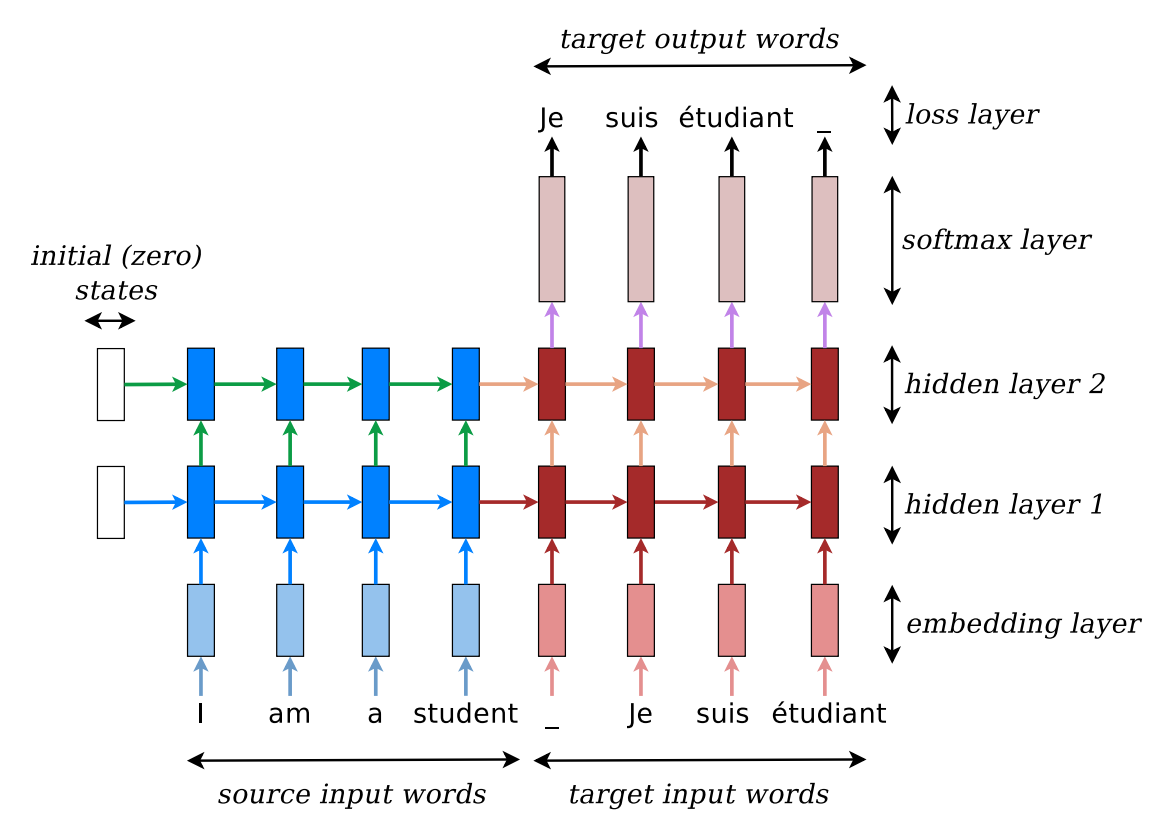
\includegraphics[width=12cm]{nmt}
	\caption{ Neural machine translation – example of a deep recurrent architecture (\cite{luong2015effective})}
	\centering
\end{figure}

The most common network structure is the encoder-decoder framework and 
\[ p(e_1^I | f_1^J) = \prod_{t} p(e_i|e_0^{i-1}, f_1^J) = \prod_{t} {p(e_i| e_{i-1}, h_{i-1}, f_1^J)} \] 


A basic form of NMT consists of two components: an encoder which computes a representation $\bm{s}$ for the whole source sentence and a decoder which generates one target word a a time and hence decomposes the conditional probability as:
\[ p(e_1^I|f_1^J) = \prod_{i=1}^{I} p(e_i| e_{i-1}, \bm{s})  \]
In more detail, the probability of decoding each word $e_i$ as:
\[ p(e_i|e_{i-1}, \bm{s}) = softmax(g(\bm{h_i}))\]
$g$ is trainable function which gives the probability of all target words in the vocabulary. 
$\bm{h}_i$ is the RNN hidden unit, abstractly computed as:
\[ \bm{h_i} = f(\bm{h}_{i-1}, \bm{s})\]
where $f$ defines the transformation connecting hidden states.  








%
%\[ p(e_t|e_{t-1} h_{t-1}, f_1^J) =  p(e_t| e_{t-1}, h_{t-1}, c_t)\]
%
%\[ \bm{\tilde{h_{t}}} = tanh(\bm{W_{c}[c_t; h_t]}) \]
%\[p(y_t| y_{<t}, x) = \text{softmax}(\bm{W_s \tilde{h_t}})\]

Drawbacks of the such seq2seq model:
\begin{enumerate}
	\item The model compresses all information from the input sentence into a hidden vector ${1}$, while ignores the length of input sentence, when the length of input sentence get very long, even longer than the training sentences, it becomes harder to extract specific information for predicting the target word, the performance will get worse.
	\item It's not suitable to assign the same weight to all input words, one target word corresponds usually to one or several words in the input sentence. Treating all words equally does not distinguish the source information and influence the performance badly.
\end{enumerate}

\subsection{Attention Mechanism}
To solve the problem mentioned above, attention mechanism was proposed to derive a context vector ${\bm{c_t}}$ that capture the input information to help to predict the target word at time ${t}$. The basic idea is: given the target hidden state ${\bm{h_t}}$ and the source-side context vector $\bm{c_t}$, we can compute the hidden state ${\tilde{\bm{h}}_i}$ by combining the current hidden state $\bm{h_t}$ and the context vector $\bm{c_t}$:
\[ \tilde{\bm{h}}_t = tanh(W_c[\bm{c_t}; \bm{h_t}])\]

Then the target word can be predicted by softmax function:
\[ p(e_i| y_{\le i, x}) = softmax(W_s \tilde{\bm{h}}_t)\] 

\begin{figure}[t]
	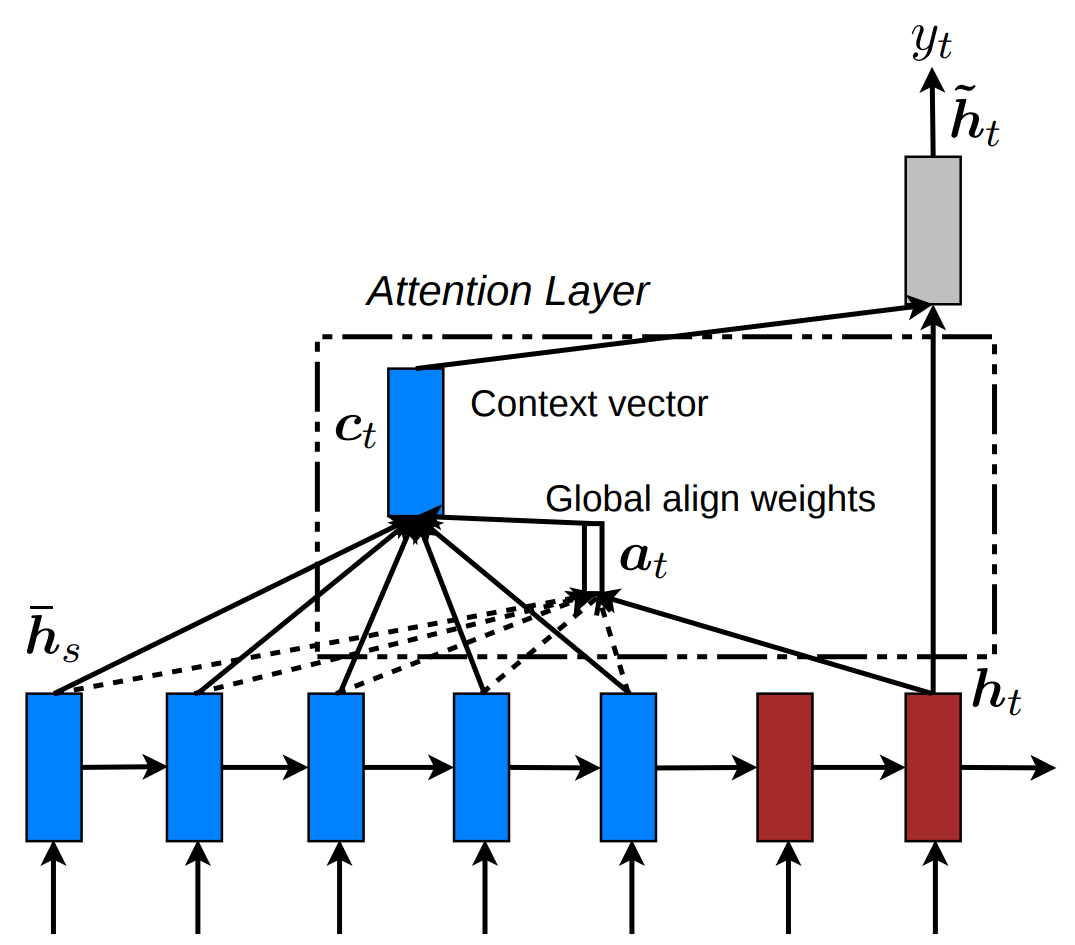
\includegraphics[width=12cm]{attentiong}
	\caption{Global attention model (\cite{luong2015effective})}
	\centering
\end{figure}

\begin{figure}[t]
	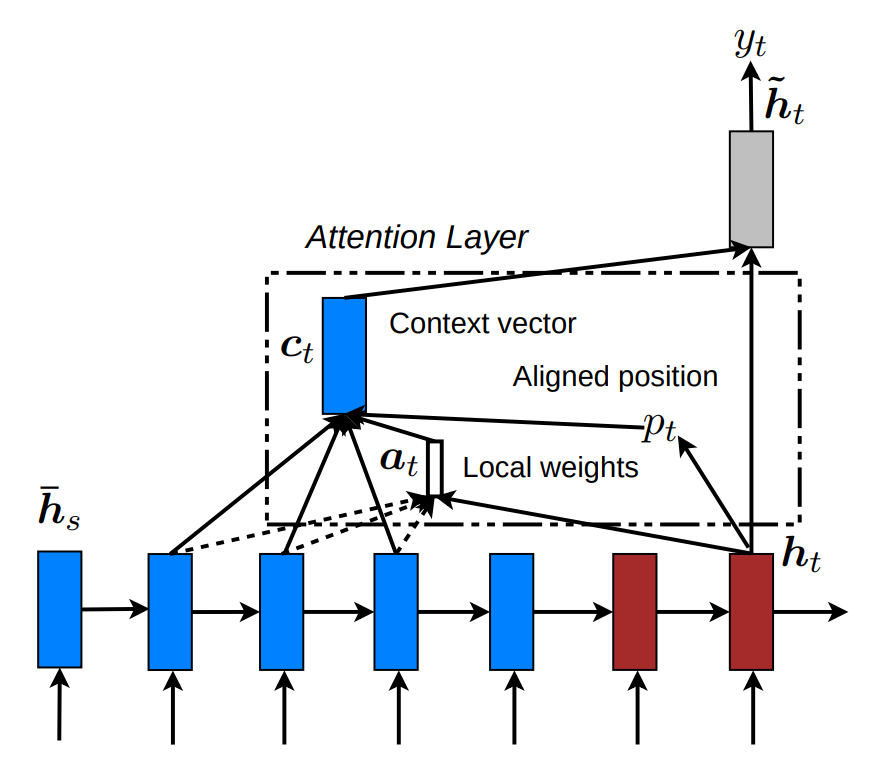
\includegraphics[width=12cm]{attentionl}
	\caption{Local attention model (\cite{luong2015effective})}
	\centering
\end{figure}
The concept of attention mechanism comes first from the computer vision domain \cite{xu2015show}, when generating image captions,  The model learns to restrict attention to particular objects in the image.

\cite{bahdanau2014neural}
\textbf{Global attention} \\
The global attention attend all the input words, weighted sum of 
\begin{align}
a_i(\bm{s}) = & \ \text{align}(\bm{h_i}, \bar{\bm{h}}_s) \\
= & \ \frac{\text{exp}(\text{score}(h_i, \bar{\bm{h}}_s))}{\sum_{\bm{s}^{\prime}} \text{exp}(\text{score}(h_i, \bar{h}_s^{\prime}))}
\end{align}

\begin{equation}
\text{score}(\bm{h_i}, \bar{\bm{h}}_s)=\left\{
\begin{array}{lcl}
{\bm{h_i}}^T \bar{\bm{h}}_s & & dot\\
{\bm{h_i}}^T W_a \bar{\bm{h}}_s & & general\\
{\bm{v_i}}^T tanh(W_a[\bm{h_i}; \bar{\bm{h}}_s]) & & concat
\end{array} \right.
\end{equation}

with soft attention you need to calculate the attention over all features, however with hard attention, it is a deterministic methods so that 
Hard attention \\
Soft attention means when computing the distribution of the alignment, for each word in the input sentence, the model will give a probability.

In comparison with the soft attention, the hard attention will determine a specific word from the input sentence as the alignment and force the alignment probability as ${0}$.  Hard attention mechanism works in image processing however it performs worse in text processing. Because such one-to-one alignment will produce bad translation once a mis-alignment occurs. \cite{luong2015effective} 


\textbf{Local attention }\\
Since for global attention, for each target word we need to attend the whole input sentence, it is very expensive and impractical to translate longer sentences. Proposed the local attention, the local attention is actually the  tradeoff between soft and hard attention, Soft attention tries to place attention over the whole image "softly" while select one patch of the image to attend. The hard attention need more complicated techniques like variance reduction or reinforcement learning though need less computation when inference.

Local attention: the model first generate an aligned position ${p_i}$ for word at the position ${i}$. Then the context vector ${\bm{c}_i}$ is a weighted sum within the window ${[p_i-D, p_i+D]}$, ${D}$ is selected empirically. The model predict the aligned  position ${p_i}$ as followed:
\[ p_i = S \cdot \text{sigmoid}(\bm{v}_p^T \text{tanh}(W_p \bm{h}_i))\]

${W_p}$ and ${\bm{v}_p}$ are the model parameters which will be learned to predict positions.
To favor the words near position ${p_i}$, we place a Gaussian distribution which centered at ${p_i}$.
\[\bm{a}_i(s) = \text{align}(\bm{h}_i, \bar{\bm{h}}_s)\text{exp}\Big(-\frac{(s-p_i)^2}{2 \sigma^2}\Big) \]

\subsection{Transformer}
\begin{figure}[t]
	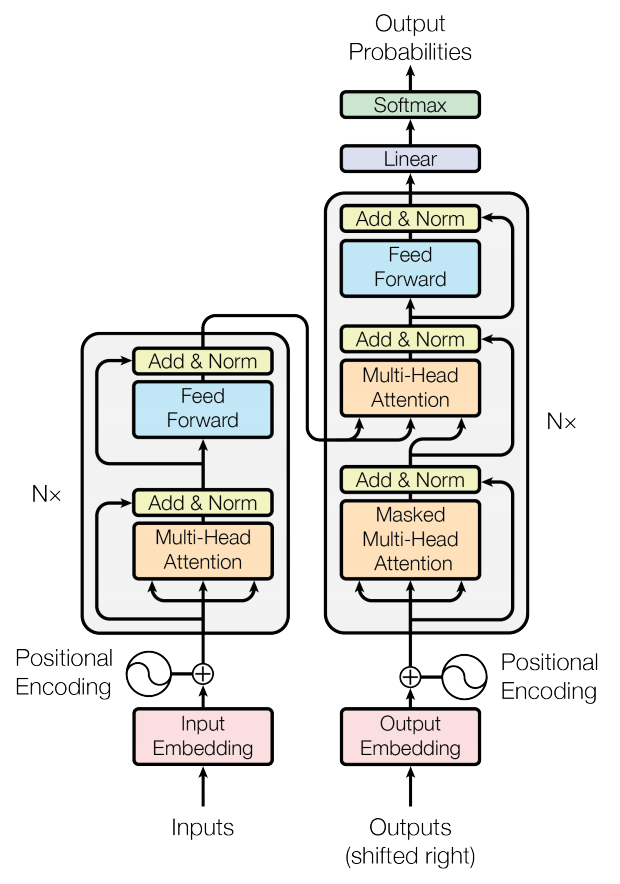
\includegraphics[width=10cm]{transformer}
	\caption{(The Transformer model architecture\cite{vaswani2017attention})}
	\centering
\end{figure}
As the illustration above, the long-short term memory (LSTM) and gated recurrent units (GRU) have achieved state of the art in sequence modling and machine translation problem. However the RNN models also have some disadvantages, because of its sequential nature, it is more difficult to fully take advantage of the modern computing devices uch GPU and TPU, which excel at parallel computation not sequential processing.


Dot-Product Attention
a query q and a set of key-value (k-v) pairs to an output, the weight of the each value is the inner product of the query and corresponding key.
Queries and keys are of the same dimension ${d_k}$, values are of dimension ${d_v}$, than the attention of query on all (k-v) pairs are:

\[ A(q, K, V) = \sum_{i}{ \frac{e^{q\cdot k_i}}{\sum_{j} e^{q\cdot k_j} v_i}}\]
When we stack the queries ${q}$ to ${Q}$:
\[ A(Q, K, V) = softmax(QK^T)V\]

As ${d_k}$ get larger, the variance of ${q^T k}$ get larger.  The softmax become very peaked and the gradient get smaller. To counteract this effect, we scaled the dot products by ${\frac{1}{\sqrt{d_k}}}$.

\[ Attention(Q,K,V) = softmax(\frac{QK^T}{\sqrt{d_k}})V\]


multi-head attention: first map $Q$,$K$,$V$ into $h$ many lower dimension spaces via linear mapping matrix. Then apply attention and concatenate the outputs. 
Suppose the original dimensions of queries, keys, values are ${d_model}$. We the number of heads is ${h}$, then ${d_k = d_v = d_{model}/h}$. With ${i \in 1 \cdots h}$ different matrix ${W_i^Q \in R^{d_{model}\times d_k}}$ ${W_i^K \in R^{d_{model}\times d_k}}$ ${W_i^V \in R^{d_{model}\times d_k}}$ and ${W^O \in R^{d_{model}\times d_k}}$.

\[ MultiHead(Q, K, V) = Concat(head_1, \cdots, head_h)W^O \]
\[head_i = Attention(QW_i^Q, KW_i^K, VW_i^V) \]


Transformer reduce the training complexity to a constant ${O(1)}$ number of operations.



The encoder-decoder attention: the queries come from the previous decoder layer, the keys and values are just the output of decoder. This works as the attention mechanism in the seq2seq model, it allow the decoder to align all positions in the input sequence with different weights

encoder self-attention: all queries, keys, values come from the encoder layer, each position allows to attend to all positions before that position.

decoder self-attention: similar to encoder attention, each position is allowed to attend to position before and including that position.


Positional Encoding
Since there is no RNN or CNN structures in transformer model, we need also need to make use of sequence information for seq2seq learning. We need inject position information into the embedding.
\[PE_{(pos, 2i)} = sin(pos/ 10000 ^{2i / d_{model}})\]
\[ PE_{(pos, 2i+1)} = cos(pos / 10000^{2i/d_{model}})\]


where pos is the position and $i$ is the dimension. That is, each dimension of 

\section{Unsupervised Machine Translation}


\subsection{Decipherment}

\[ \argmax{\theta} \prod_{f} \sum_{e} P(e) \cdot P_{\theta}(f|e)\]

for hidden alignments: \[ \argmax{\theta} \prod_{f} \sum_{e} P(e) \cdot \sum_{a} P_{\theta}(f,a|e) \]


Propose a simple generative story for MT without parallel data. The model accounts for word substitutions, insertions, deletions and local reordering during the translation process but does not incorporate fertilities or global re-ordering.

The generative process:
\begin{enumerate}
	\item Generate an English sentence $e_1^N$ with probability $P(e)$.
	\item Insert a NULL word at any position in the English sentence with uniform probability.
	\item For each English word token $e_i$ (including NULLs), choose a foreign word translation $f_i$, with probability $P_{\theta}(f_i| e_i)$, the foreign word may be NULL.
	\item Swap any pair of adjacent foreign words $f_{i-1}, f_i$, with probability ${P_{\theta}(swap)}$. 
	\item Output the foreign string $f_1^M$, skipping over NULLs.
\end{enumerate}

use the Expectation Maximization (EM) algorithm to estimate $\theta$ in order to maximize likelihood of the foreign corpus. Finally use the Viterbi algorithm to decode the foreign corpus. and Produce an English translation $e_1^N$ that maximizes ${P(e_1^N)\cdot P_{\theta}(f_1^M | e_1^N)}$ but EM training face some problems, EM cannot scale to such large vocabulary sizes, need to instantiate the entire channel and resulting derivation lattice before we can run EM, this is too big to be stored in memory. Introduce iterative EM: identify the top K frequent word types in both the English and foreign data. Replace all the other word tokens with ‘UNK’, use EM algorithm to train this model to maximize likelihood of cipher data. Then extend the vocabulary size from K to 2K and so on.
Iterative EM
\cite{nuhn2012deciphering}
%Since it is not feasible to deal with the full parameter table, add more constraints: for each foreign word ${f}$, number the candidates words ${e^{\prime}}$ with $p(f|e^{\prime}) > 0$ is below a fixed value, he tries to determine the set of active lexicon entries by exploiting monolingual context similarity. Further in his work, to speed up the computation speed. Beam search: look at $B_{LM}$ many successor words ${e_{n+1}}$ with highest LM probability ${p_{LM}(e_{n+1}| e_n)}$ and $B_{lex}$ many successor words with high probability ${p_{lex}(f_{n+1}|e_{n+1})}}$.
Altogether only look at ${B_{LM}+B_{lex}}$ many successor states.
\cite{nuhn2014decipherment}


\cite{gehring2017convolutional}
\subsection{Neural Unsupervised Machine Translation}

\begin{algorithm}[H]
	\SetAlgoLined
	\KwResult{Unsupervised Machine Translation}
	\KwIn{Language models ${LM_{s}}$ ${LM_t}$ over the source and target languages} 
	\textbf{Initialize translation models:}  Leveraging ${P_s}$ and ${P_t}$, learn two initial translation models, one in each direction: ${P_{s\rightarrow t}^{(0)}}$ and ${P_{t\rightarrow s}^{(0)}}$ 
	\BlankLine
	\For{${k=1}$ to ${N}$}{
		\begin{itemize}
			\BlankLine
			\item   \textbf{Backtranslation:} Generate source and target sentences using the current
			translation models ${P_{t\rightarrow s }^{(k-1)}}$ and ${P_{s \rightarrow t}^{(k-1)} }$, factoring in language models, ${P_s}$ and ${P_t}$;
			\item   \textbf{Train new translation models ${P_{s\rightarrow t}^{(k)}}$ and ${P_{t \rightarrow s}^{(k)}}$:} Use the generated sentences and leveraging ${P_s}$ and ${P_t}$
		\end{itemize}
	}   
\end{algorithm}
The key idea is to build a common latent space between the two languages (or domains) and to learn to translate by reconstructing in both domains according to two principles. 



They initialize the model with an inferred bilingual dictionary. They leverage strong language model: denoising autoencoder,  third, they implemented the back translation: the key idea is to train two translation models which translate in contrary directions at the same time. The last property is that the models constrain the latent representations produced by the encoder to be shared between the two languages. The encoders will encoder the input into a common latent representation space independent of the language. The decoder plays the role of translator and will try to learn to improve the translation quality with the help of back translation mechanism.

\subsubsection{Dual Structure}
made an important contribution. They train two agents to translate in opposite directions (e.g. French $\rightarrow$ English and English $\rightarrow$ French), and make them teach each other through a reinforcement learning process. While promising, this approach still requires a parallel corpus for a warm start.

\subsubsection{Initialization}
\textbf{Denoising autoencoder} Initialize the algorithm by using a naive unsupervised translation model based on a word-by-word translation of the sentence with a bilingual lexicon derived from the same monolingual data. While such initial "word-by-word" translation maybe poor if languages or corpora are not closely related, it still preserves some of the original semantics
%\log P_{t\rightarrow t}(e|\text{noise}(e)
%\log P_{s\rightarrow s}(f|\text{noise}(f)) 
\subsubsection{Optimization}
\textbf{Denoising autoencoder}\\
by minimization 
\[ L^{auto} = \mathbb{E}_{e\sim E}[-\log P_{t\rightarrow t}(e|\text{noise}(e)] + \mathbb{E}_{f\sim F} [-\log P_{s\rightarrow s}(f|\text{noise}(f))]\]
where $s$ $P_{s\rightarrow s}$ and $P_{t\rightarrow t}$ are the composition of encoder and decoder both operating in the source and target sides, respectively.
\textbf{Back-Translation}\\
Since we have dual structure for bi-directional translation, we denote the sentence that translated by intermediate target-to-source translation model as $u(y)$, similarly denote the sentence translated by source-to-target model as $v(x)$, so $u(y)$ should in source language and $v(x)$ should in target language. The pairs $(x, v(x))$, $(u(y), y)$ constitute synthetic parallel  sentences. They can be used to train the two machine translation models by minimizing the back-translation loss:
\[ L^{back} = \mathbb{E}_{y\sim T} [-\log P_{s\rightarrow t}(y|u(y))] +  \mathbb{E}_{x\sim S} [-\log P_{t\rightarrow s}(x|v(x))]\]

The objective functipn minimized at every iteration of stochastic gradient descent is simply the sum of $L^{auto}$ and $L^{back}$. 
\textbf{Shared Latent Representation} 
A shared encoder representation actis like an interlingua, which is translated in the decoder corresponding language regardless less of the input source language.  
\begin{itemize}
	\item Shared encoder
	The system use only one encoder that is shared by both languages involved. The universal encoder is aimed to produce a language independent representation of the input language but the decoder should separately translate then into corresponding language.
	\item Adversarial training
	Train discriminator to classify between the encoding of source and target sentences. The discriminator operates on the output of the encoder, the encoder is trained instead to fool the discriminator. 
\end{itemize}








